\chapter{Experimentos}
\label{cap:capitulo6}

En este capítulo se recogen las distintos experimentos que se han llevado a cabo durante el desarrollo del proyecto. Estas pruebas han sido fundamentales para verificar el correcto funcionamiento del sistema de reconocimiento de maduración de frutos y su comunicación con el brazo robótico, permitiendo así alcanzar los objetivos definidos en fases anteriores del trabajo.

\section{Selección del algoritmo de detección y bibliotecas}
\label{exp_seleccion_algoritmo}

Dada la finalidad del proyecto, se requería que la detección de objetos se diera en tiempo real, por lo que se buscó información sobre YOLO, un sistema de código abierto que permitía esto a partir de una red neuronal convolucional para detectar objetos en imágenes.\\

Después de realizar la lectura \textit{You Only Look Once: Unified, Real-Time Object Detection} \cite{Redmon16}, se replicó lo que se exponía en dicho artículo con la webcam del ordenador portátil, mediante un programa en Python y usando la librería Open Source Computer Vision Library (OpenCV) mediante la biblioteca Pytorch. Este programa, partiendo del feed de la propia webcam, descomponía el vídeo en imágenes o cuadros, alimentando a la red neuronal (en este caso YOLOv3), que recibía esta detección y se procesaba con OpenCV, dibujando los recuadros o \textit{bounding box} alrededor de los objetos que se detectaban en vivo.
Para esto, primero se realizó la instalación de OpenCV, instalando Anaconda para poder crear un ambiente y así evitar problemas entre las versiones de los paquetes necesarios al clonar el repositorio con el código y los actuales, mientras se siguieron los pasos detallados en el archivo README.
Una vez instalado todo, se probó a utilizar varios objetos y posteriormente varias frutas simultáneamente para ver si el modelo las diferenciaba correctamente y las detectaba.

  \begin{figure}[H]
    \begin{center}
      \subcapcentertrue
      \subfigure[Prueba deteccion de objetos con Pytorch]{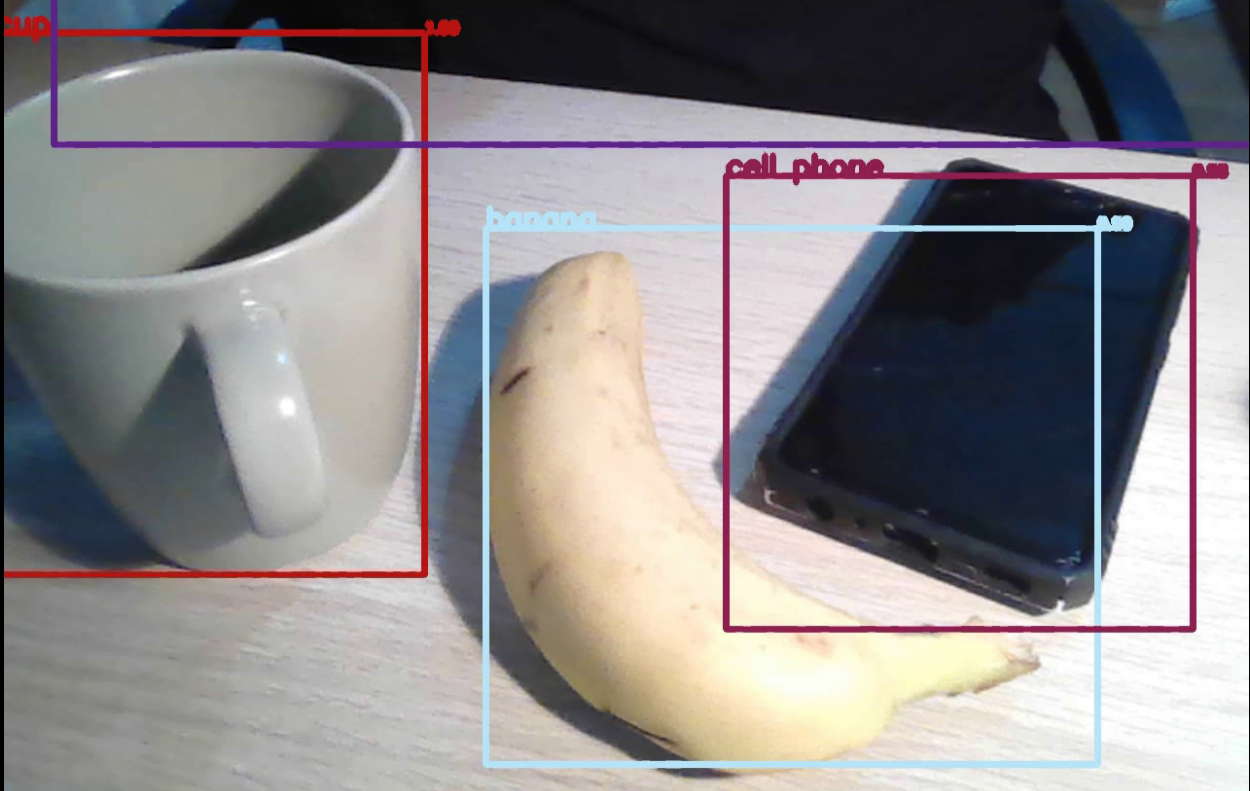
\includegraphics[width=73mm]{figs/Prueba deteccion de objetos con pytorch.png}}
      \hspace{2mm}
      \subfigure[Prueba deteccion de frutas con Pytorch]{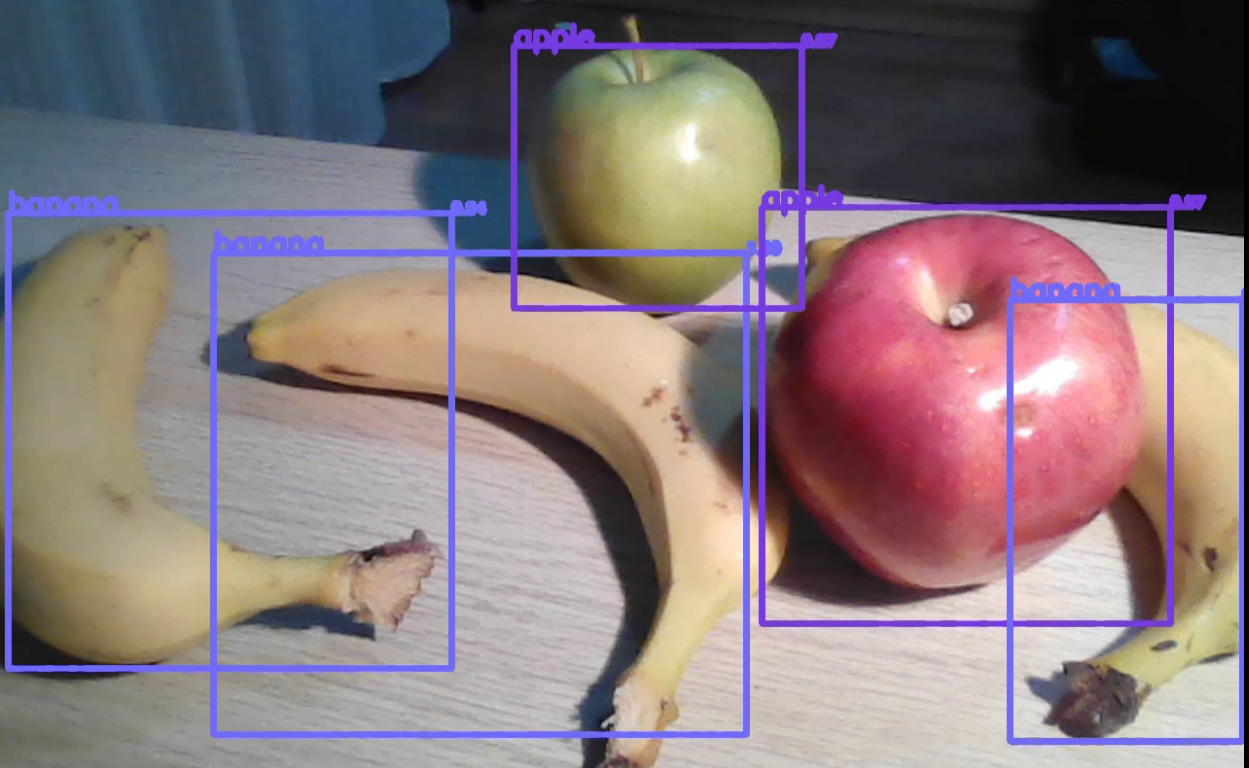
\includegraphics[width=75mm]{figs/Prueba derteccion de frutas con pytorch.png}}
    \end{center}
    \caption{Deteccion con Pytorch}
    \label{fig:Deteccion_Pytorch}
  \end{figure}

Para poder comprobar las diferencias en un ejemplo práctico a la hora de detectar objetos entre PyTorch y TensorFlow, y de esta manera poder escoger una de las dos bibliotecas para el desarrollo del modelo de aprendizaje automático y aprendizaje profundo en este proyecto, se decidió crear de nuevo un entorno de Anaconda y empezar a probar a detectar objetos en imágenes. Para esto, se siguieron los pasos del repositorio de deteccion objetos\footnote{\url{https://github.com/puigalex/deteccion_objetos}} basados en la configuración faster rcnn resnet101 coco de los modelos de detección de objetos de Tensorflow.

Para esto, se llevó a cabo el etiquetado de las imágenes mediante la herramienta labelImg\footnote{\url{https://github.com/HumanSignal/labelImg}} y se prepararon las carpetas y archivos de configuración correspondientes para poder llevar a cabo el entrenamiento del modelo siguiendo los pasos indicados en el repositorio. 
Se puede observar en la siguiente imagen como al iniciar este entrenamiento la pérdida era demasiado alta y existían demasiadas fluctuacionessin ningún problema.

\section{Detección de fresas en imágenes con TensorFlow}
\label{exp_fresas_Tensorflow}

Dado el éxito obtenido con el ejemplo de los tigres, se propuso comprobar si el modelo funcionaría también con el objeto final, en este caso, con las fresas. Para ello, se obtuvo a través de la página Kaggle un dataset de 262 frutas de las cuales únicamente se utilizó el archivo de las fresas, que contenía 1002 imágenes.

Una vez descargado el archivo, se comenzó a etiquetar una a una las imágenes mediante la herramienta labelImg para obtener los archivos xml, tal y como se había hecho con el anterior ejemplo.

Antes de terminar de etiquetar el dataset entero, se intentó probar este modelo. Para ello, en esta ocasión se siguió uma distribución de las primeras 405 imágenes del 80:20 (80 datos de entrenamiento y 20 datos de prueba).

Tras repetir los diferentes pasos explicados anteriormente para entrenar el modelo, cortándolo esta vez en el paso 3501, y usando el checkpoint guardado en el paso 3490 para congelar el modelo. Finalmente se utilizaron varias imágenes aún por etiquetar para probarlo, obteniendo un resultado satisfactorio

